\chapter{EMPATÍA}
El presente capítulo desarrolla la primera etapa del Design Thinking aplicada al presente proyecto: Empatizar. Esta fase tiene como propósito comprender en profundidad las necesidades, motivaciones y frustraciones de los jóvenes respecto a su experiencia con las redes sociales y la conexión emocional digital, complementando la evidencia documental presentada en el Capítulo 3 con evidencia primaria recolectada directamente del grupo objetivo. Para ello se aplicaron cuatro técnicas, a partir de las plantillas de Design Thinking en Español: el Análisis Dimensional, para encuadrar el reto; el Guion de entrevista cualitativa; las Entrevistas cualitativas, aplicadas a seis participantes; y la Técnica de los 5 ¿Por qué?, para profundizar en las causas raíz de los problemas identificados.

\section{ANÁLISIS DIMENSIONAL}
El Análisis Dimensional es una técnica de análisis estratégico cuyo objetivo es asegurar que se conoce el reto que se va a abordar, mediante la respuesta a seis preguntas que permiten dimensionar el problema; en Design Thinking se aplica como punto de partida, durante la fase de Empatía (Design Thinking en Español, s.f.-a). Su aplicación al presente proyecto arrojó los siguientes resultados:

\begin{itemize}
    \item \textbf{¿Cuál es el problema?} Los jóvenes están hiperconectados, pero emocionalmente desconectados: acumulan muchos contactos con poca conexión real, mantienen interacciones superficiales y un consumo pasivo de contenido, en plataformas que priorizan los \textit{likes} sobre los vínculos, lo que genera una brecha entre la cantidad de conexiones y la calidad del vínculo.
    \item \textbf{¿Quiénes están involucrados?} Los jóvenes de 16 a 28 años, incluidos aquellos que no son conscientes de su desconexión; sus familiares y círculo cercano; las plataformas de redes sociales; y la investigadora y desarrolladora del proyecto.
    \item \textbf{¿Para qué resolverlo?} Para mejorar la calidad de las conexiones digitales de los jóvenes, favorecer la regulación emocional mediante micro interacciones, reducir la brecha entre la hiperconectividad y el bienestar real, y promover comunidades digitales más empáticas.
    \item \textbf{¿Qué grado de relevancia tiene el problema?} Alta: un meta-análisis con 81,344 adolescentes y jóvenes adultos encontró una asociación moderada y consistente entre el uso problemático de las redes sociales y una mayor soledad (Feng et al., 2026), y la soledad se asocia con una peor calidad del sueño y con mayor morbilidad y mortalidad (Hawkley \& Cacioppo, 2010).
    \item \textbf{¿Cuál es la causa?} Plataformas que incorporan elementos de diseño orientados a prolongar el tiempo de uso y no a mejorar la calidad del vínculo (Montag et al., 2019); métricas públicas y un uso pasivo que favorecen la comparación social (Verduyn et al., 2017); y la falta de interacción recíproca y personalizada, que es la que se asocia con mejoras en el bienestar (Burke \& Kraut, 2016).
    \item \textbf{¿En qué lugar acontece el problema?} En el entorno digital, principalmente en redes sociales y aplicaciones de mensajería. El proyecto se desarrolla en Cochabamba, Bolivia, pero el problema se validó mediante entrevistas a jóvenes de Bolivia, Chile, España y Ecuador (sección 4.3).
\end{itemize}

\section{GUÍA DE LA ENTREVISTA CUALITATIVA}
Con el objetivo de establecer una guía de apoyo para orientar el desarrollo de las entrevistas, se elaboró un guion estructurado en tres momentos: introducción, preguntas personales, y dos bloques temáticos centrales (redes sociales y bienestar emocional), cerrando con una conclusión. Siguiendo la técnica de Guion de entrevista cualitativa, el guion incluye los temas sobre los que se busca profundizar y, por cada tema, preguntas abiertas que permiten identificar problemas, necesidades, deseos o comportamientos de los usuarios (Design Thinking en Español, s.f.-c). El diseño de este instrumento se fundamentó en los factores de desconexión emocional identificados en el Capítulo 3, particularmente aquellos vinculados al tipo de interacción digital (Godard \& Holtzman, 2024; Liu et al., 2026), a la comparación social (Verduyn et al., 2017) y a la brecha entre la cantidad de contactos y la calidad de los vínculos (Hawkley \& Cacioppo, 2010; Burke \& Kraut, 2016). La Figura \ref{fig:guion_entrevista} presenta el guion completo utilizado en las entrevistas.

\begin{figure}[htbp]
  \centering
  \caption{Guion de la entrevista cualitativa}
  \label{fig:guion_entrevista}
  \vspace{4pt}
  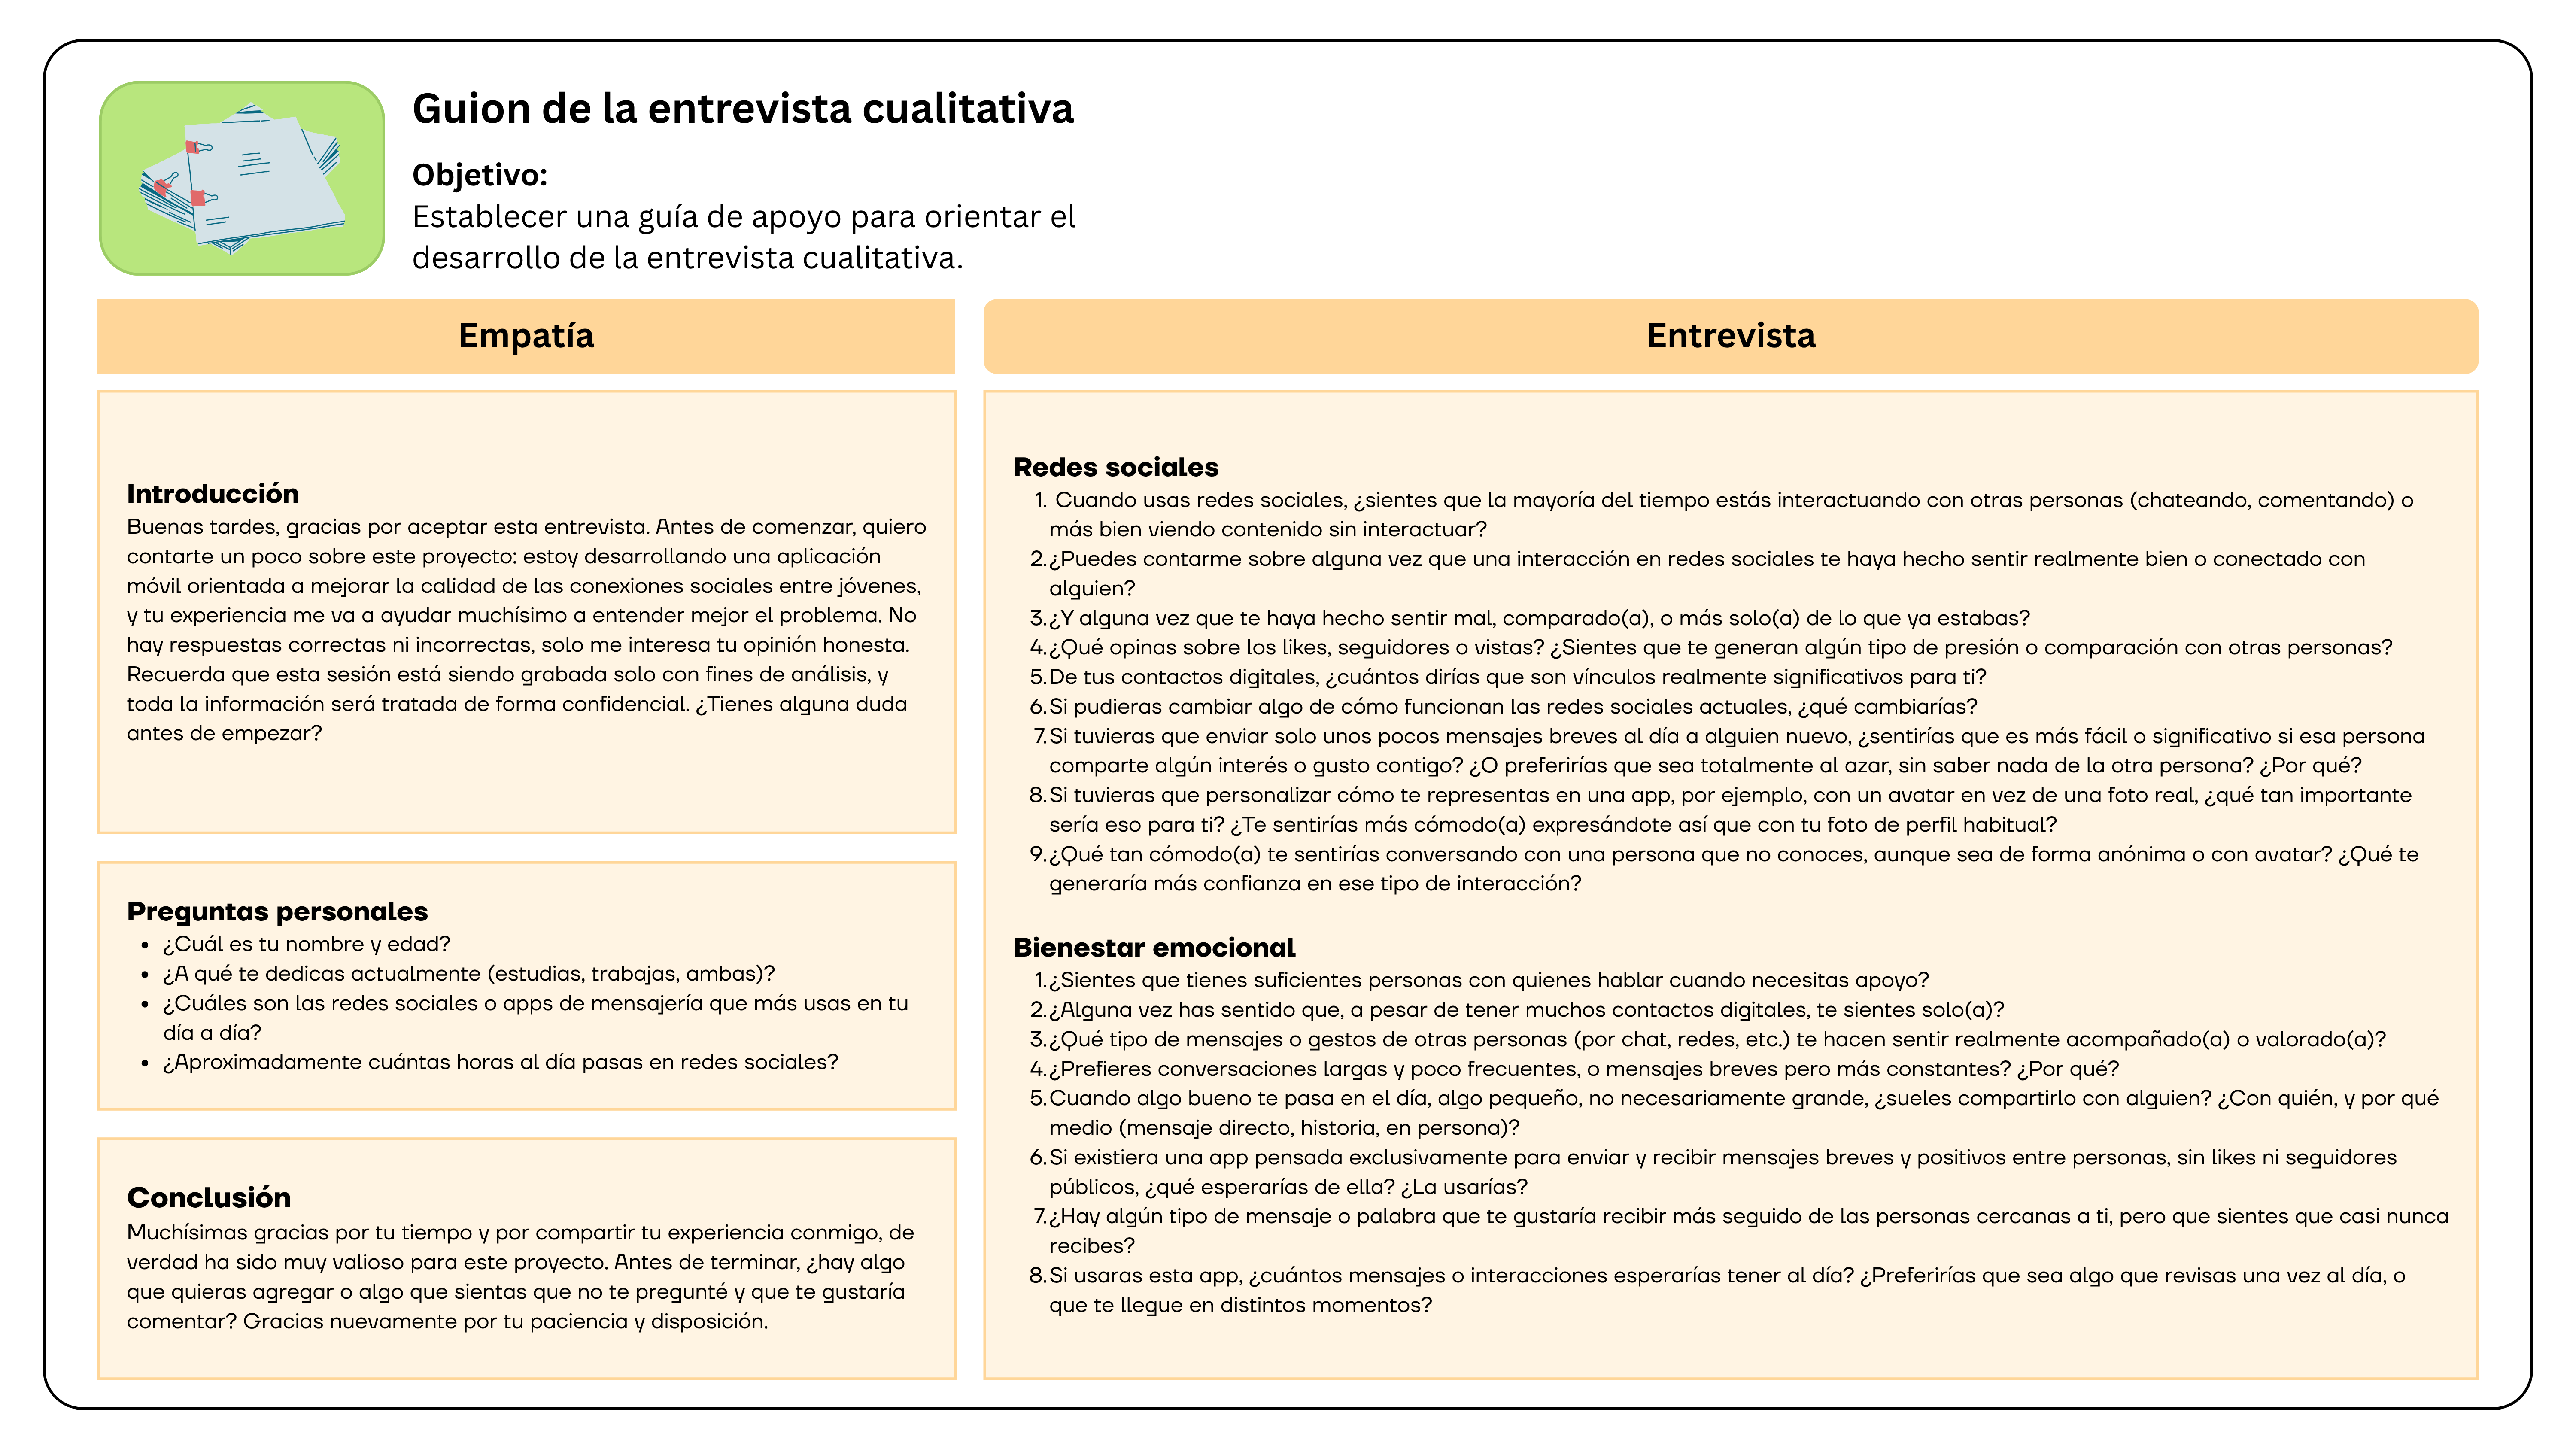
\includegraphics[width=0.95\textwidth]{Images/stages/Qualitative-interview-guide.png}
  \vspace{4pt}
\end{figure}

\section{APLICACIÓN DE LAS ENTREVISTAS}
La guía descrita fue aplicada a seis jóvenes de entre 20 y 28 años (Usuario 1: Rolando Mercado Rojas, Usuario 2: Rubén Hernández Torrez, Usuario 3: Fernando José Pérez Armando, Usuario 4: Antonia Tapia, Usuario 5: Alejandra Pérez Ramal, Usuario 6: Renata Martínez Mitte), reclutados a través de grupos digitales de contacto directo con el grupo objetivo. Los participantes provienen de cuatro países: Bolivia (Usuarios 1 y 2), Chile (Usuarios 3 y 4), España (Usuario 5) y Ecuador (Usuario 6). Cuatro de ellos son estudiantes y dos trabajan (Usuarios 2 y 3); el Usuario 5 prefirió no indicar su edad. La inclusión de participantes de distintos países amplía la diversidad de perspectivas, aunque implica que los hallazgos no se circunscriben únicamente al contexto boliviano. El criterio de selección priorizó la diversidad de perfiles (género, nivel de sociabilidad autopercibido) con el fin de enriquecer los hallazgos cualitativos y comprender, como proponen Vargas Márquez et al. (2021), las necesidades físicas y emocionales de los usuarios y lo que es significativo para ellos (p. 12). Las entrevistas tuvieron una duración aproximada de 20 a 30 minutos cada una, y sus resultados fueron sistematizados utilizando la técnica de Entrevistas cualitativas, que busca obtener información sobre las experiencias reales de los usuarios (Design Thinking en Español, s.f.-b), organizada en cuatro categorías: necesidades, problemas, deseos y observaciones.

A continuación, se presentan de forma detallada los resultados de los Usuarios 1 y 4, seleccionados por representar perfiles contrastantes dentro de la muestra (un perfil introvertido con dificultad de vinculación frente a uno sociable con red de apoyo consolidada), lo cual permite ilustrar la amplitud de experiencias recogidas.

\subsection{Usuario 1}
El Usuario 1, de 25 años, estudiante universitario, presenta un uso moderado de redes sociales (1 a 2 horas diarias). Se define a sí mismo como una persona reservada e introspectiva, con dificultad para iniciar y mantener conversaciones tanto digitales como presenciales.

\begin{figure}[htbp]
  \centering
  \caption{Entrevista cualitativa - Usuario 1}
  \label{fig:entrevista_usuario1}
  \vspace{4pt}
  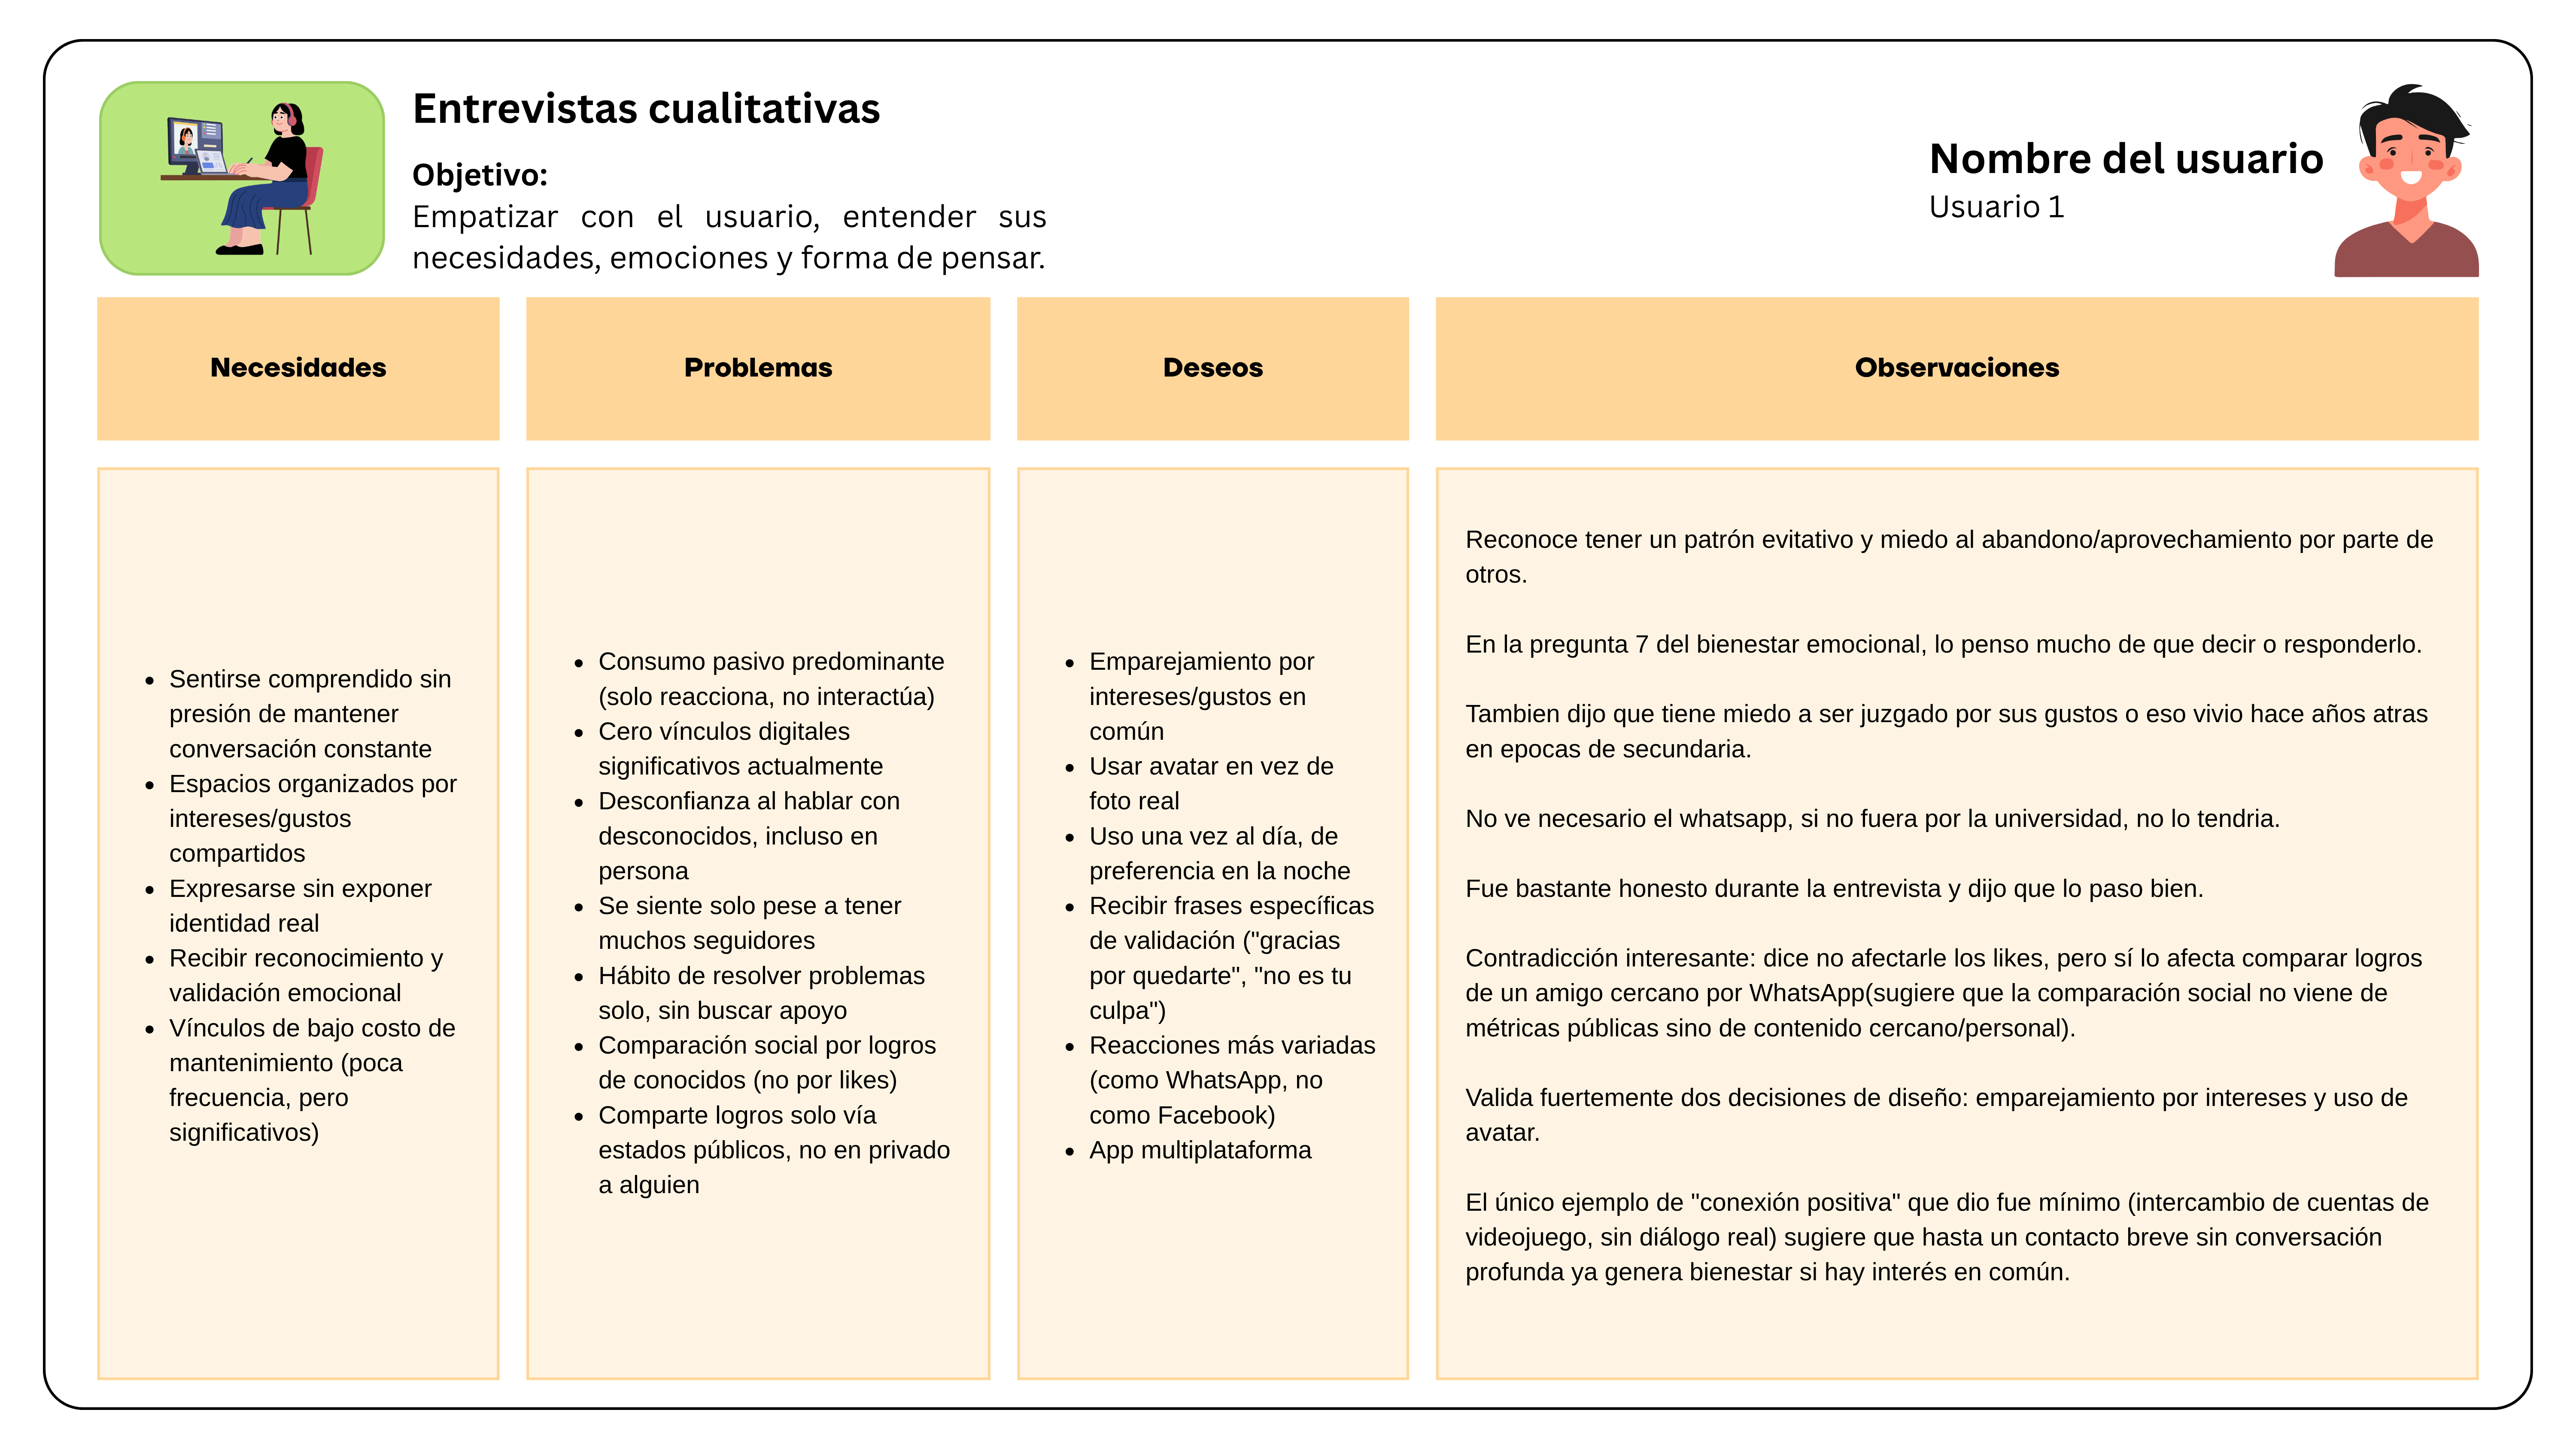
\includegraphics[width=0.9\textwidth]{Images/methodology/empathy/usuario1EC.png}
  \vspace{4pt}
\end{figure}

Entre los hallazgos más relevantes de esta entrevista destaca que el Usuario 1 no identifica ningún vínculo digital que considere significativo, pese a contar con un número considerable de seguidores en redes sociales, lo que ilustra que la soledad depende de la calidad de las relaciones y no solo de su cantidad (Hawkley \& Cacioppo, 2010), en coherencia con los hallazgos de Burke y Kraut (2016), según los cuales el bienestar no se asocia con las interacciones rápidas o dirigidas a audiencias amplias, sino con la comunicación personalizada entre vínculos fuertes. Asimismo, valida fuertemente dos decisiones de diseño relevantes para el presente proyecto: la preferencia por el emparejamiento basado en intereses compartidos, consistente con el meta-análisis de Montoya et al. (2008), según el cual la similitud real entre personas se asocia con la atracción interpersonal ($r = .47$), especialmente en interacciones breves o iniciales, y el uso de un avatar en lugar de una fotografía real como medio de expresión.

\subsection{Usuario 4}
El Usuario 4, de 20 años, estudiante, presenta un uso considerable de redes sociales (3 horas diarias). A diferencia del Usuario 1, cuenta con una red de apoyo sólida y vínculos significativos ya establecidos, mostrando un perfil más sociable, aunque igualmente crítico frente a las dinámicas actuales de las redes sociales.

\begin{figure}[htbp]
  \centering
  \caption{Entrevista cualitativa - Usuario 4}
  \label{fig:entrevista_usuario4}
  \vspace{4pt}
  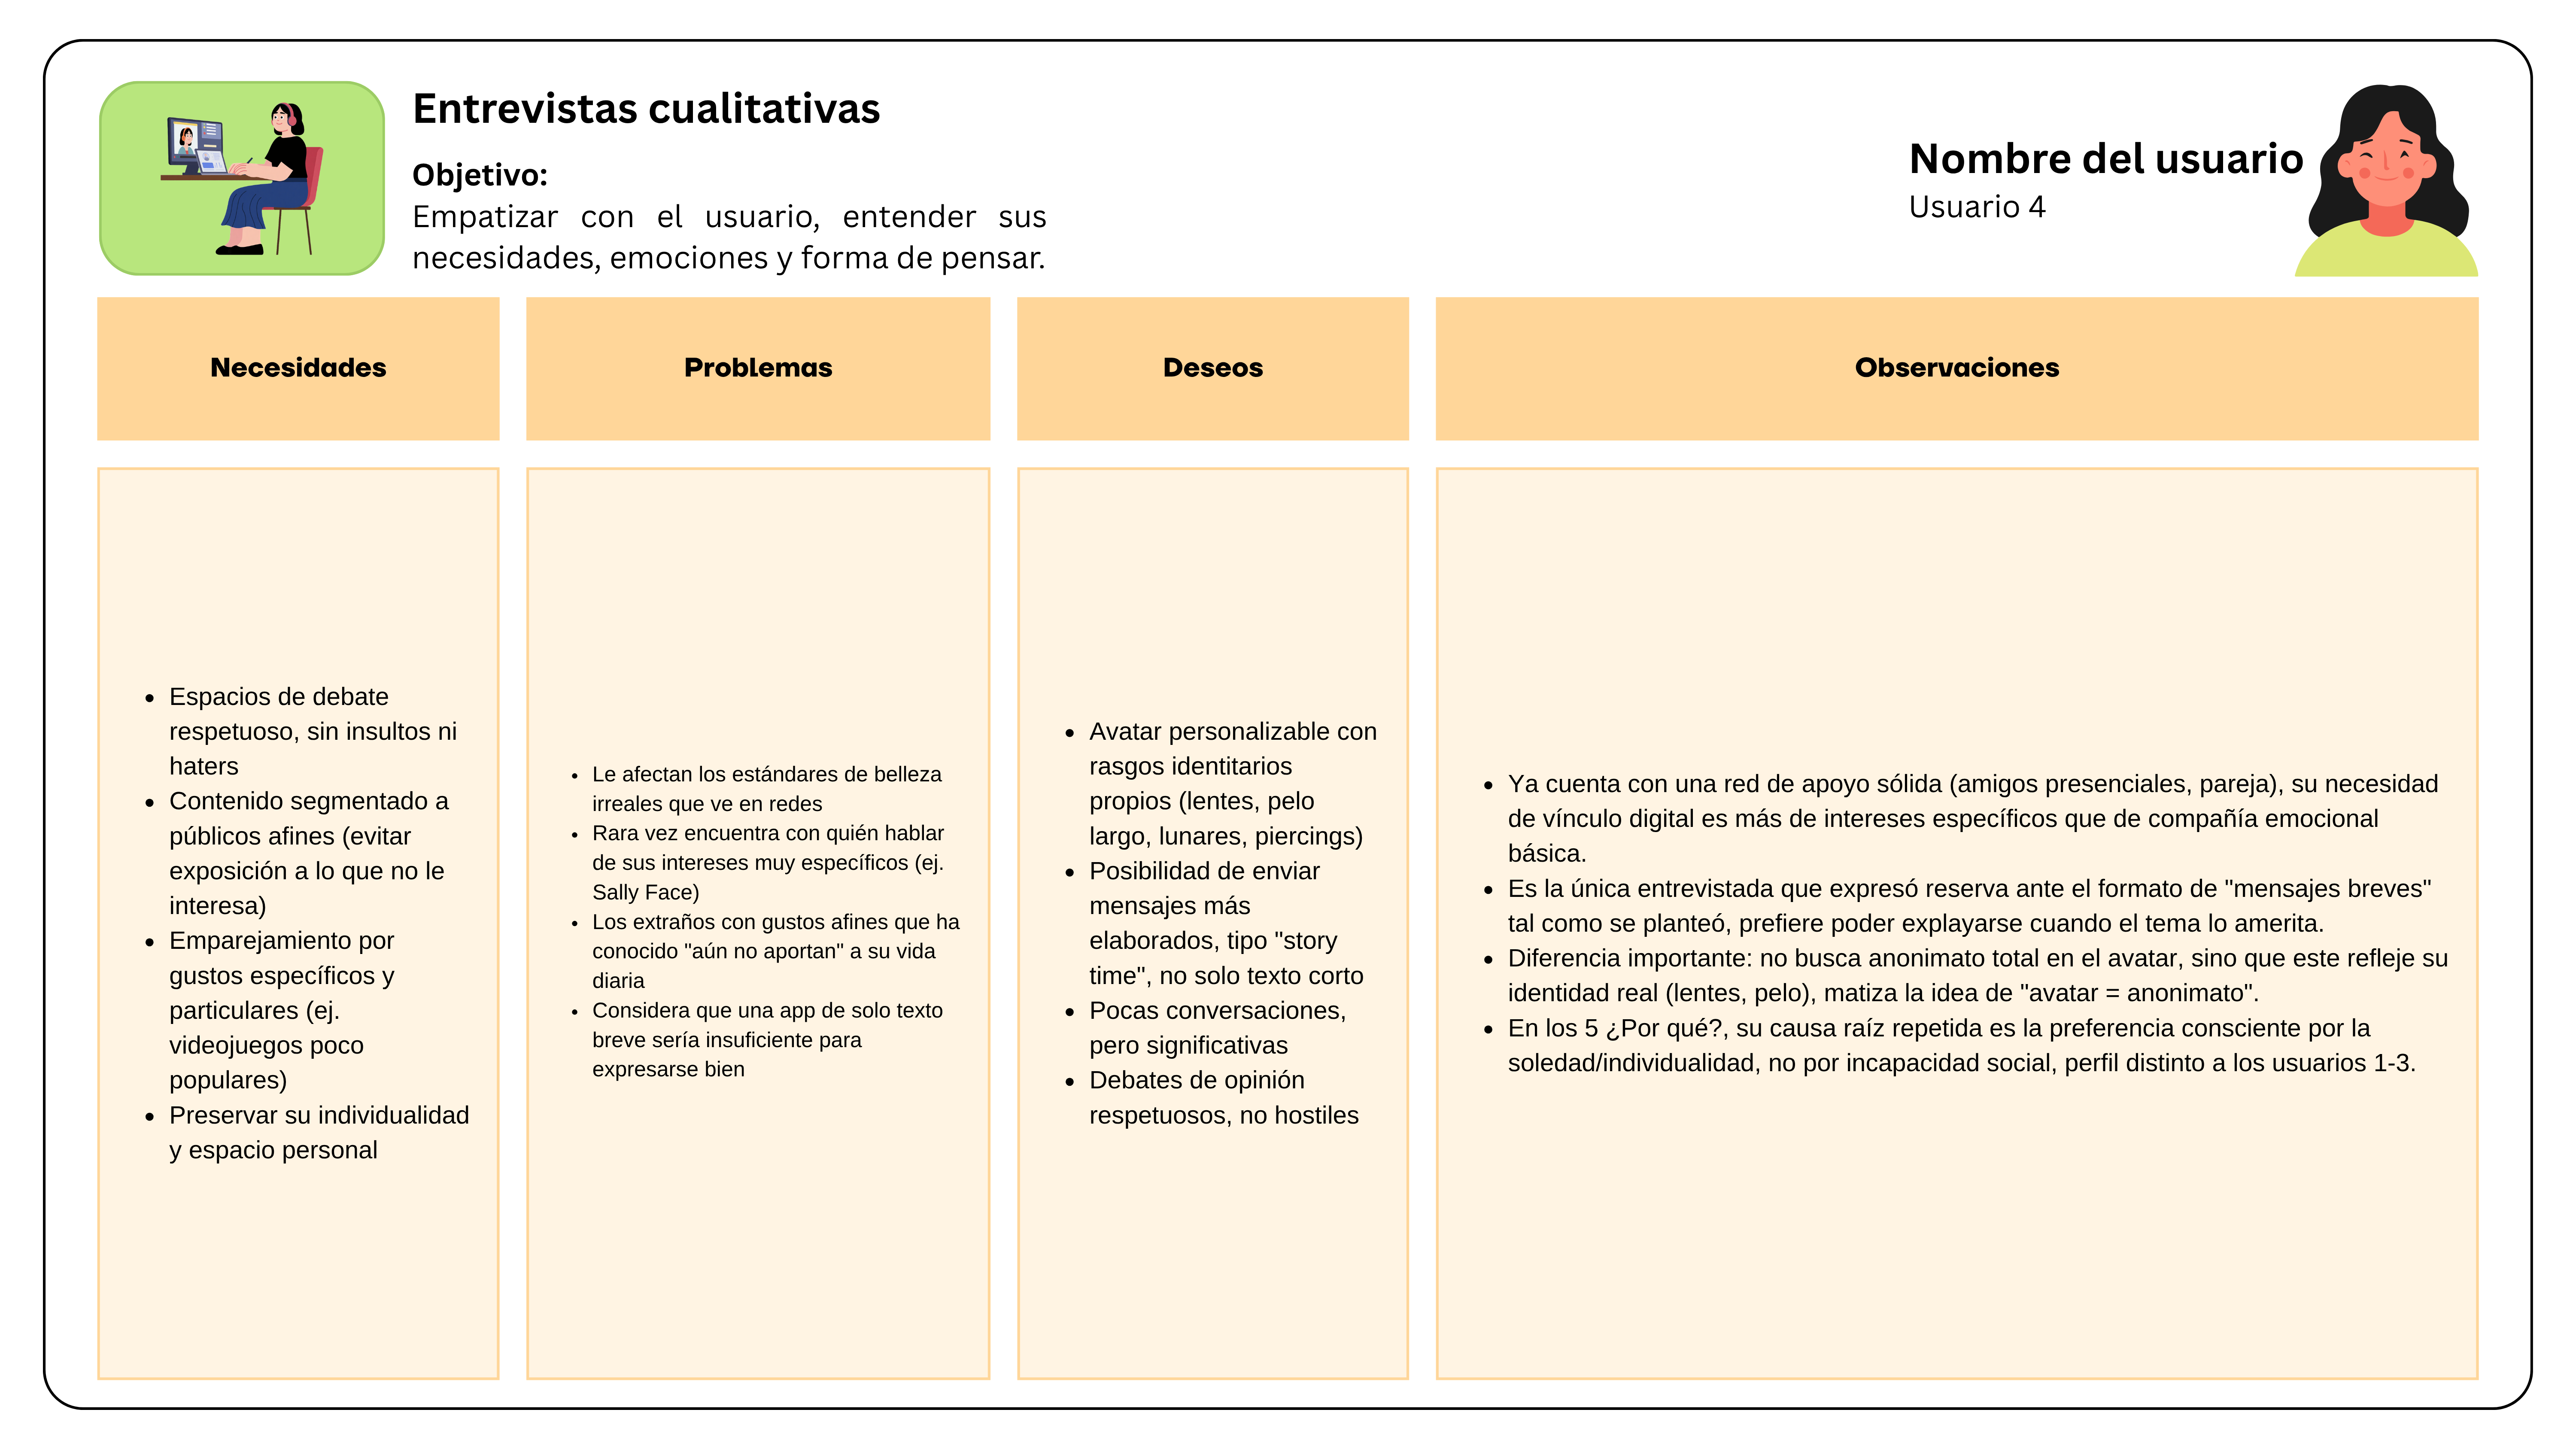
\includegraphics[width=0.9\textwidth]{Images/methodology/empathy/usuario4EC.png}
  \vspace{4pt}
\end{figure}

El Usuario 4 expresó reservas respecto al formato de mensajes exclusivamente breves, señalando que en ocasiones necesita mayor espacio para expresarse. Este hallazgo resulta relevante frente al concepto de micro interacciones sociales positivas de Saffer (2013), pues sugiere que la brevedad, si bien valiosa como principio general, no debe aplicarse de forma rígida para todos los perfiles de usuario. Asimismo, destacó la importancia de que el avatar refleje rasgos identitarios reales, matizando la idea inicial de que el avatar debía funcionar como anonimato total.

\subsection{Usuarios 2, 3, 5 y 6}
De manera complementaria, el mismo instrumento fue aplicado a los Usuarios 2, 3, 5 y 6. El Usuario 2 (23 años, trabajador, Bolivia) considera algo significativos solo uno o dos de sus vínculos digitales, suele esperar que otros inicien la conversación y ha presenciado un trato hostil hacia personas nuevas en comunidades en línea; además, se mostró escéptico frente a la aplicación propuesta. El Usuario 3 (28 años, vendedor, Chile) cuenta con dos o tres vínculos digitales significativos, necesita un tema en común para sentirse cómodo conversando y expresa temor a confiar en alguien y que esa persona termine aprovechándose. El Usuario 5 (estudiante, España) afirma contar con varias personas de apoyo y, aun así, experimentar soledad en ocasiones, y valora los espacios libres de toxicidad y el resguardo de su privacidad. El Usuario 6 (21 años, estudiante, Ecuador) cuenta con un solo vínculo digital significativo, tras haber perdido otro sin entender la razón, y expresa temor a interactuar con desconocidos de malas intenciones.

De forma consistente con los Usuarios 1 y 4, estos cuatro participantes reportaron dificultades para sostener vínculos digitales significativos, preocupación por la hostilidad o la desconfianza hacia desconocidos en línea, y una valoración positiva del emparejamiento por intereses compartidos y del uso de avatares como medio de expresión. Estos resultados son coherentes con el meta-análisis de Feng et al. (2026), según el cual la soledad se asocia con mayor fuerza al uso problemático de las redes sociales que al tiempo de exposición, y con una definición de la soledad centrada en la calidad de las relaciones, que explica que pueda presentarse incluso cuando se cuenta con apoyo (Hawkley \& Cacioppo, 2010).

\section{TÉCNICA DE LOS 5 ¿POR QUÉ?}
Con el objetivo de profundizar en las causas raíz de los problemas identificados durante las entrevistas, se aplicó la Técnica de los 5 ¿Por qué?, que consiste en volver a preguntar ``¿Por qué?'' cinco veces consecutivas ante cada respuesta para llegar a los motivos profundos del comportamiento o pensamiento de la persona (Design Thinking en Español, s.f.-h). La técnica se aplicó a cuatro problemas recurrentes: la soledad pese a tener múltiples contactos digitales, el predominio del consumo pasivo sobre la interacción activa, la comparación social generada por likes y seguidores, y la dificultad para generar conversaciones significativas con desconocidos. Esta técnica permitió superar la descripción superficial de los síntomas para llegar a explicaciones más profundas, en coherencia con la recomendación de Vargas Márquez et al. (2021) de preguntar siempre ``¿Por qué?'', ya que ``eso descubre nuevos significados'' (pp. 11--12).

A continuación, se presentan los resultados detallados de los Usuarios 1 y 5, seleccionados por ilustrar dos causas raíz distintas y complementarias entre sí.

\subsection{Usuario 1}
\begin{figure}[htbp]
  \centering
  \caption{Técnica de los 5 ¿Por qué? - Usuario 1}
  \label{fig:5porque_usuario1}
  \vspace{4pt}
  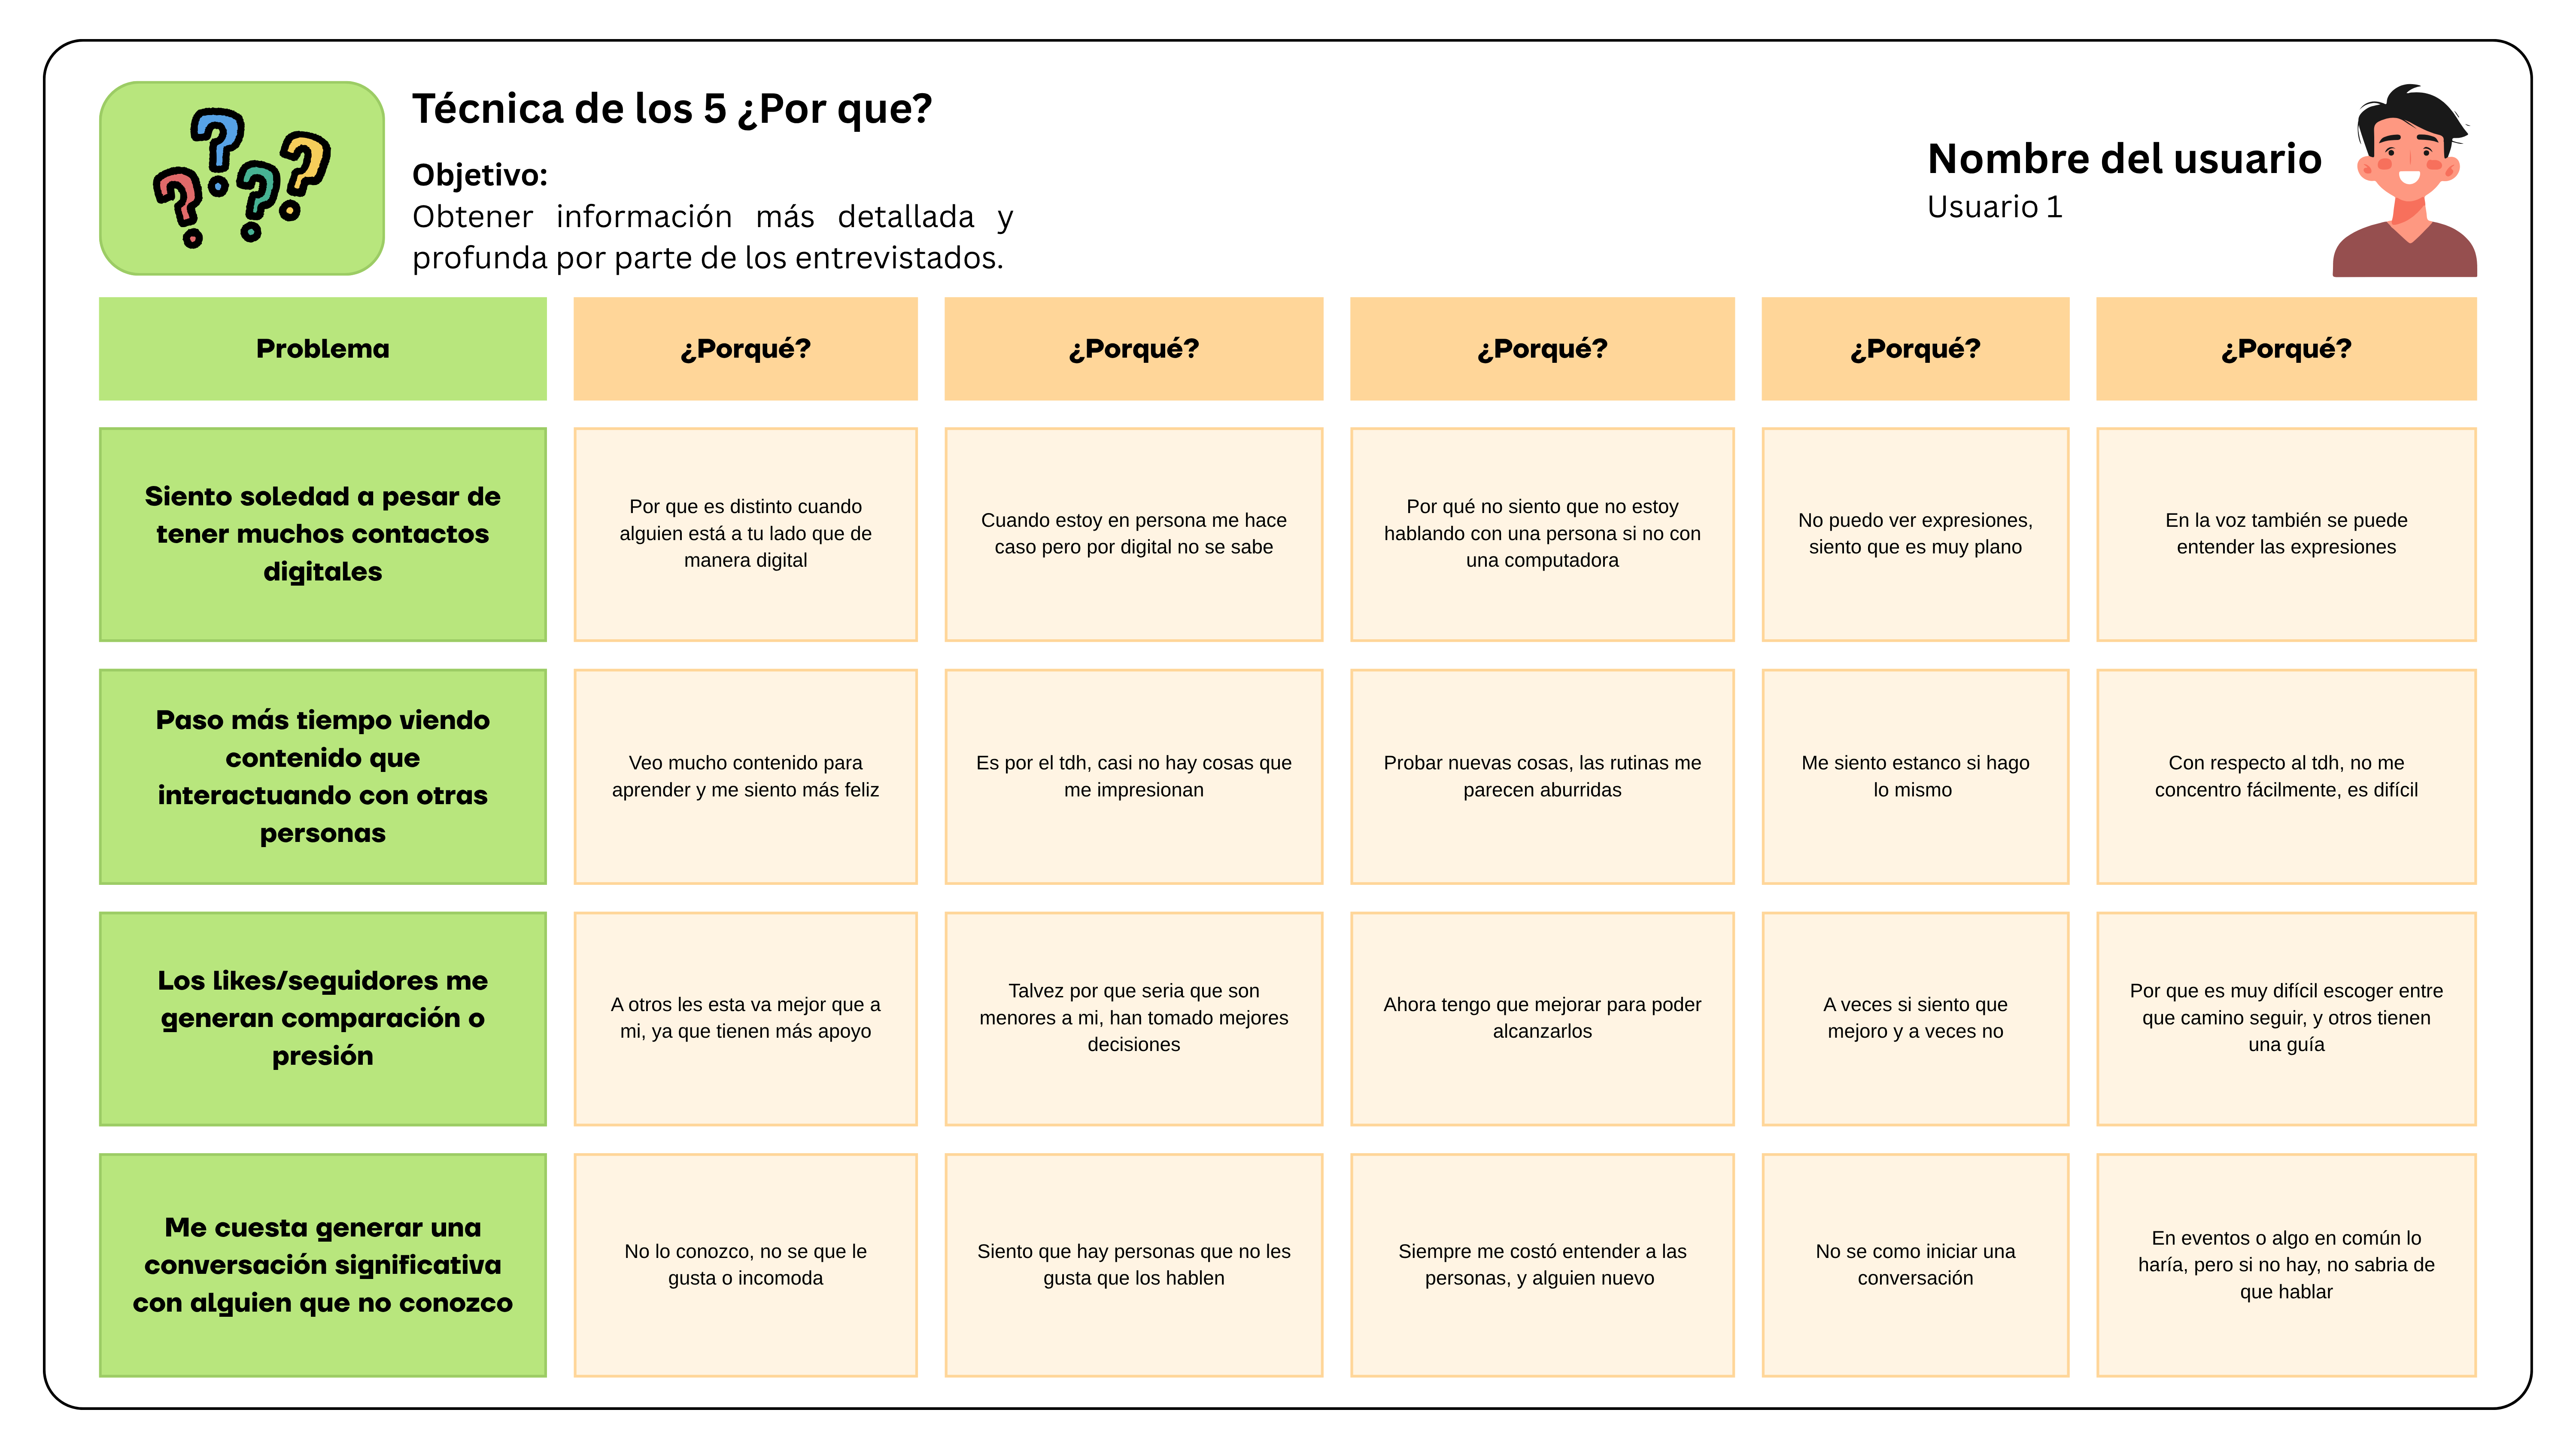
\includegraphics[width=0.9\textwidth]{Images/methodology/empathy/usuario1-5P.png}
  \vspace{4pt}
\end{figure}

El análisis reveló que, para el Usuario 1, la causa raíz de la desconexión digital radica en la ausencia de señales no verbales en la comunicación en línea, lo que hace que la interacción se perciba como poco genuina en comparación con el contacto presencial. Este hallazgo es coherente con lo señalado por Picard (1997), quien observa que la comunicación textual prescinde de la entonación de la voz y de la expresión facial (p. 13), y con la falta de señales no verbales identificada por Tufail et al. (2025) en la comunicación de jóvenes universitarios en redes sociales.

\subsection{Usuario 5}
\begin{figure}[htbp]
  \centering
  \caption{Técnica de los 5 ¿Por qué? - Usuario 5}
  \label{fig:5porque_usuario5}
  \vspace{4pt}
  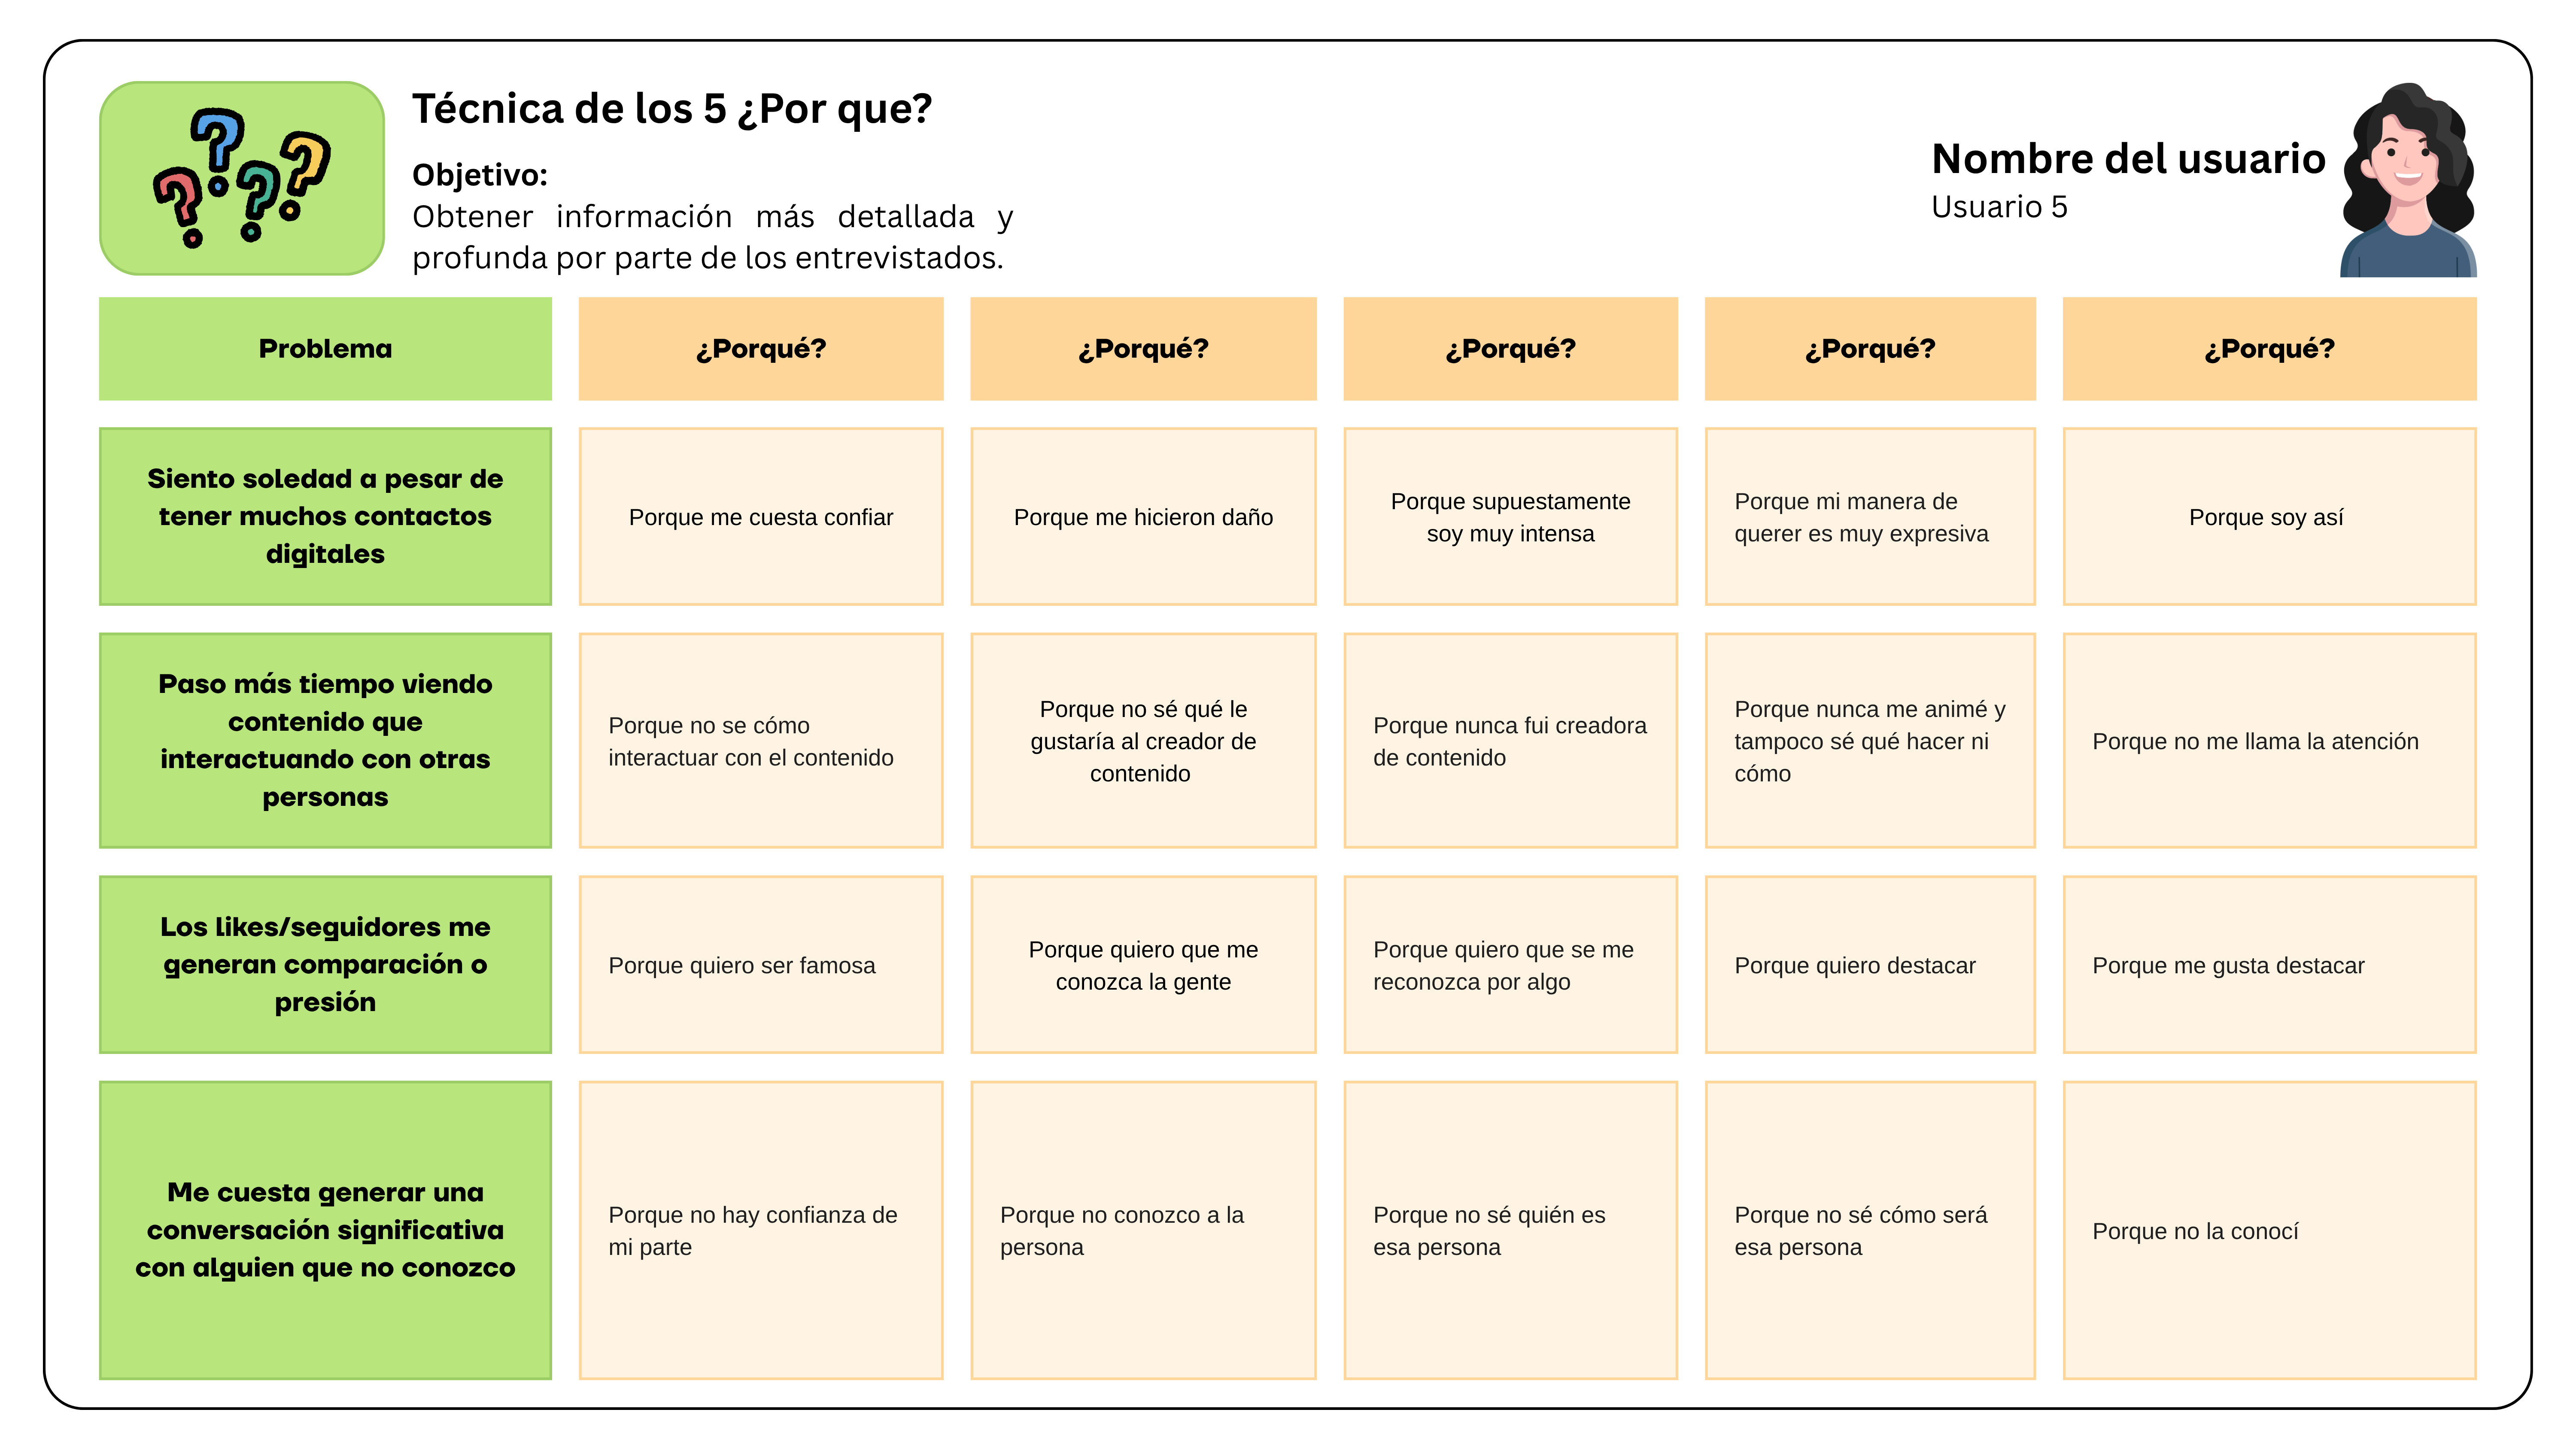
\includegraphics[width=0.9\textwidth]{Images/methodology/empathy/usuario5-5P.png}
  \vspace{4pt}
\end{figure}

En este caso, la causa raíz identificada se vincula a experiencias previas de conflicto derivadas de una forma intensa y expresiva de relacionarse, lo que ha generado cierta cautela al momento de establecer nuevos vínculos digitales. Este hallazgo puede interpretarse desde el modelo de proceso de la regulación emocional de Gross (1998b), particularmente en lo referido a la selección de la situación, ya que la cautela al establecer nuevos vínculos funciona como una forma de evitar situaciones que podrían resultar emocionalmente intensas.

\subsection{Usuarios 2, 3, 4 y 6}
El mismo análisis fue aplicado a los Usuarios 2, 3, 4 y 6. En los Usuarios 2, 3 y 6, las causas raíz coinciden en tres ejes: la falta de confianza inicial hacia desconocidos (en el Usuario 3, por temor a que la otra persona termine aprovechándose), la ausencia de un tema o interés en común que facilite el inicio de la conversación (Usuarios 2, 3 y 6), y el temor a que la conversación no funcione o a que los propios temas no resulten interesantes para el otro (Usuarios 2 y 6). El Usuario 4 presenta un patrón distinto: sus causas raíz remiten a una preferencia consciente por la individualidad y el espacio personal (``porque estoy tranquila con mi individualidad''), y no a una dificultad para vincularse. Los ejes identificados son coherentes con la caracterización de la soledad como la percepción de que las necesidades sociales no están siendo satisfechas, especialmente por la calidad de las relaciones (Hawkley \& Cacioppo, 2010), y con la noción de ``ilusión de la amistad significativa en línea'' documentada por Parry et al. (2026).

\section{SÍNTESIS DE LA FASE EMPATIZAR}
La aplicación de las técnicas descritas en el presente capítulo permitió confirmar, desde la evidencia primaria, los factores identificados previamente a partir de la literatura en el Capítulo 3. De manera consistente entre los seis participantes, se evidenció: (a) la existencia de vínculos digitales numerosos pero de bajo significado emocional, en línea con Burke y Kraut (2016) y Parry et al. (2026); (b) una fuerte preferencia por el emparejamiento basado en intereses o gustos compartidos como facilitador de la conversación, consistente con Montoya et al. (2008); (c) una valoración positiva del uso de avatares como medio de expresión frente a la exposición de la identidad real; (d) una necesidad explícita de mecanismos que generen confianza y seguridad frente a la interacción con desconocidos; y (e) una comparación social que surge principalmente del contenido de otras personas (logros de conocidos, videos de personas exitosas o estándares de belleza) más que de las métricas propias de \textit{likes} o seguidores (Usuarios 1, 3, 4 y 6), lo que coincide con el planteamiento de que el uso pasivo de las redes sociales provoca comparaciones sociales y envidia (Verduyn et al., 2017). Estos hallazgos constituyen la base para la construcción del planteamiento del problema y la definición del punto de vista de diseño que se desarrolla en el Capítulo 5.